\begin{name}
	{\tenchude}
	{\tendethi}
	{\tentruong}
	{Life isn’t about finding yourself. Life is about creating yourself}
\end{name}
\Opensolutionfile{ansbook}[ans/ansbookDe1]
\TN
\Opensolutionfile{ans}[ans/ansDe1-TN1]\begin{ex}%[1D6N1-1]%[Dự án đề kiểm tra Toán 11 CHKII NH23-24- Ngô Tất Thành]%[THPT Phạm Văn Sáng - Tp HCM]
Cho biểu thức $P=\sqrt[4]{x^3}$, $(x>0)$. Mệnh đề nào dưới đây \textbf{đúng}?
\choice
{$P=x^{\frac{4}{3}}$}
{\True $P=x^{\frac{3}{4}}$}
{$P=x^{\frac{4}{6}}$}
{$P=x^{\frac{6}{4}}$}
\loigiai{
Ta có $P=\sqrt[4]{x^3}=x^{\frac{3}{4}}$.
}
\end{ex}

\begin{ex}%[10-11EX-GK2-2425]%[Quan Ón]%[1D6N2-2]
Cho $P = \log_{a}a^2b^{10}$ với $a>0$, $b>0$. Tìm khẳng định đúng.
\choice
{$P = 12\log_{a}b$}
{$P = 20\log_{a}b$}
{\True $P = 2 + 10\log_{a}b$}
{$P = 2\log_{a}b$}
\loigiai{
Ta có $P = \log_{a}a^2b^{10} = \log_{a}a^2 + \log_{a}b^{10} = 2 + 10\log_{a}b$.
}
\end{ex}

\begin{ex}%[1D6N3-1]%[Dự án C đợt 3 - Khắc Thiên]
Với $a$ là số thực dương bất kì, mệnh đề nào dưới đây \textbf{đúng}?
\choice
{\True $\log a^3=3\log a$}
{$\log (3a)=\dfrac{1}{3} \log a$}
{$\log (3a)=3\log (a)$}
{$\log a^3=\dfrac{1}{3} \log a$}
\loigiai{Dựa vào tính chất của logarit $\log a^{\alpha}=\alpha \log a$.}
\end{ex}

\begin{ex}%[1H8N1-1]
Trong không gian, cho đường thẳng $d$ và điểm $O$. Qua $O$ có bao nhiêu đường thẳng vuông góc với đường thẳng $d$?
\choice
{$3$}
{\True vô số}
{$1$}
{$2$}
\loigiai{
Trong không gian, có vô số đường thẳng qua một điểm cho trước và vuông góc với một đường thẳng cho trước.	}
\end{ex}

\begin{ex} %[1H8N2-1]
Cho hình chóp $S.ABC$ có cạnh bên $SA$ vuông góc với mặt phẳng $(ABC)$. Góc giữa đường thẳng $SC$ và mặt đáy là
% \begin{center}
% \begin{tikzpicture}[scale=0.5]
% % Định nghĩa các điểm
% \coordinate (A) at (0,0);
% \coordinate (B) at (2,-2);
% \coordinate (C) at (5,0);
% \coordinate (S) at ($(A)+(0,5)$);

% % Vẽ các đoạn thẳng
% \draw (S) -- (A);
% \draw (S) -- (B);
% \draw (S) -- (C);
% \draw (A) -- (B);
% \draw (B) -- (C);

% % Vẽ đoạn thẳng đứt nét
% \draw[dashed] (A) -- (C);

% % Ghi chú các điểm
% \node at (B) [below] {B};
% \node at (C) [below] {C};
% \node at (S) [above] {S};
% \node at (A) [left] {A};

% \end{tikzpicture}
% \end{center}
\choice
{$\widehat{SCB}$}
{$\widehat{SAC}$}
{\True$\widehat{SCA}$}
{$\widehat{SBC}$}
\loigiai{Ta có $SA \perp (ABC) \Rightarrow AC$ là hình chiếu của $SC$ lên $(ABC)$.\\
$\Rightarrow (SC;(ABC)) = (SC;AC) = \widehat{SCA}$.}
\end{ex}

\begin{ex}%[1H8N4-1]
Hãy chọn khẳng định đúng.
\choice
{Nếu hai mặt phẳng vuông góc với nhau thì bất cứ đường nào nằm trong mặt phẳng này cũng vuông góc với mặt phẳng kia}
{Nếu hai mặt phẳng cùng vuông góc với mặt phẳng thứ ba thì giao tuyến của chúng vuông góc với mặt phẳng thứ ba đó}
{\True Nếu mặt phẳng này chứa một đường thẳng mà đường thẳng đó vuông góc với mặt phẳng kia thì hai mặt phẳng đó vuông góc với nhau}
{Nếu mặt phẳng này chứa một đường thẳng mà đường thẳng đó vuông góc với một đường thẳng nằm trong mặt phẳng kia thì hai mặt phẳng đó vuông góc với nhau}
\loigiai{
Nếu mặt phẳng này chứa một đường thẳng mà đường thẳng đó vuông góc với mặt phẳng kia thì hai mặt phẳng đó vuông góc với nhau.
}
\end{ex}

\begin{ex}%[1H8N6-1]%[Dự án TLDT 11 Toán Từ Tâm]%[Trương Đăng Khoa]
Cho đường thẳng $a$ cắt mặt phẳng $(P)$ tại điểm $A$ và đường thẳng $a$ không vuông góc với mặt phẳng $(P)$. Trên đường thẳng $a$ lấy điểm $M$ khác $A$. Gọi $H$ là hình chiếu của $M$ trên $(P)$. Trong các phát biểu sau, phát biểu nào \textbf{đúng}?
\choice
{\True Hình chiếu vuông góc của đường thẳng $a$ trên $(P)$ là đường thẳng $AH$}
{Hình chiếu vuông góc của đường thẳng $a$ trên $(P)$ là đường thẳng đi qua $M$}
{Hình chiếu vuông góc của đường thẳng $a$ trên $(P)$ là đường thẳng đi qua $H$ và song song với $a$}
{Hình chiếu vuông góc của đường thẳng $a$ trên $(P)$ là đường thẳng đi qua $H$ và vuông góc với $a$}
\loigiai
{Hình chiếu vuông góc của đường thẳng $a$ trên $(P)$ là đường thẳng $AH$.
}
\end{ex}

\begin{ex}%[Dự án C THPTQG 2025]%[Vương Quốc Phong]%[1H8N7-1]
Cho khối chóp có diện tích mặt đáy $B$ và thể tích $V$. Chiều cao của khối chóp đã cho là
\choice
{\True $h=\dfrac{3V}{B}$}
{$h=\dfrac{1}{3} V \cdot B$}
{$h=\dfrac{V}{B}$}
{$h=\dfrac{V}{3B}$}
\loigiai{
Ta có $V=\dfrac{1}{3} B\cdot h \Leftrightarrow h=\dfrac{3V}{B}$.
}
\end{ex}

\begin{ex}%[Trần Xuân Hòa]%[1D9N1-1]
Cho hai biến cố $A$ và $B$, nếu việc xảy ra hay không xảy ra của biến cố $A$ không làm ảnh hưởng tới xác suất xảy ra của biến cố $B$ thì hai biến cố $A$ và $B$ được gọi là
\choice
{Xung khắc}
{Đối nhau}
{\True Độc lập}
{Hợp nhau}
\loigiai{
Hai biến cố $A$ và $B$ được gọi là độc lập.}
\end{ex}

\begin{ex}.%[1D9N2-1]
Cho hai biến cố A và B. Biến cố hợp của A và B là biến cố
\choice
{\lq\lq A và B xảy ra\rq\rq }
{\True \lq\lq A hoặc B xảy ra\rq\rq }
{\lq\lq A xảy ra\rq\rq }
{\lq\lq B xảy ra hoặc cả A và B xảy ra\rq\rq }
\loigiai{
Dựa vào định nghĩa.}
\end{ex}

\begin{ex}    %[1D7N1-1]
Cho hàm số $y = f(x)$ xác định trên $\mathbb{R}$ thỏa mãn $\lim\limits_{x\to 3}\dfrac{f(x)-f(3)}{x-3}=2$. Kết quả nào sau đây đúng?
\choice
{$f'(2)=3$}
{$f'(x)=2$}
{\True $f'(3)=2$}
{$f'(x)=3$}
\loigiai{
Theo định nghĩa đạo hàm của hàm số tại một điểm ta có $\lim\limits_{x\to 3}\dfrac{f(x)-f(3)}{x-3}=f'(3)=2$.
}
\end{ex}

\begin{ex}%[1D7N3-1]
Cho hàm số $y=u\cdot v$ trong đó $u$, $v$ là các hàm số có đạo hàm cấp hai. Hãy chọn khẳng định đúng.
\choice
{$y''=u'' \cdot v'+u' \cdot v''$}
{$y''=(u' \cdot v')'$}
{$y''=u'' \cdot v+u \cdot v''$}
{\True $y''=u'' \cdot v+2u' \cdot v'+u \cdot v''$}
\loigiai{
Ta có $y'=u' \cdot v+u \cdot v'$ nên $y''=u'' \cdot v+2u' \cdot v'+u \cdot v''$.
}
\end{ex}
\TNTF
\begin{ex}%[1D7H2-3]%[Dự án đề kiểm tra Toán 11 HKII NH23-24-Đợt 16- Trịnh Văn Cảnh]%[THPT Đống Đa- Hà Nội]
Cho hàm số $y=e^{x^3+3x+1}$
\choiceTF
{\True $y'=e^{x^3+3x+1} \cdot\left(3 x^2+3\right)$}
{Phương trình tiếp tuyến của đồ thị hàm số tại điểm có hoành độ $x_0=0$ là $d\colon y=3 e x-e$}
{\True Phương trình $y'=3e\cdot\left(x^2+1\right)$ có nghiệm duy nhất}
{Có $6$ giá trị nguyên của tham số $m$ để bất phương trình $y'\geq 2mx \cdot e^{x^3+3x+1}$ nghiệm đúng $\forall x \in \mathbb{R}$}
\loigiai{
\begin{itemchoice}
\itemch \textbf{Đúng.}\\
Ta có $y'=(x^3+3x+1)'\cdot e^{x^3+3x+1}=e^{x^3+3x+1}\cdot\left(3x^2+3\right)$.
\itemch \textbf{Sai.}\\
Ta có $y'(0)=3e$ và $y(0)=e$.\\
Phương trình tiếp tuyến của đồ thị tại điểm có hoành độ $x_0=0$ là\\
\[y=y'(0)(x-0)+y(0)=3ex+e.\]
\itemch \textbf{Đúng.}\\
Xét phương trình \begin{eqnarray*}
& & y'=3e\cdot\left(x^2+1\right)\\
&\Leftrightarrow & e^{x^3+3x+1}\cdot\left(3x^2+3\right)=3e\cdot\left(x^2+1\right)\\
&\Leftrightarrow & e^{x^3+3x+1}=e\\
&\Leftrightarrow & x^3+3x+1=1\\
&\Leftrightarrow & x(x^2+3)=0\\
&\Leftrightarrow & x=0.
\end{eqnarray*}
Vậy phương trình $y'=3e\cdot\left(x^2+1\right)$ có nghiệm duy nhất.
\itemch \textbf{Sai.}\\
Bất phương trình
\begin{eqnarray*}
& & y'\geq 2mx \cdot e^{x^3+3x+1}, \forall x\in \mathbb{R}\\
&\Leftrightarrow & 3x^2+3\geq 2mx, \forall x\in \mathbb{R}\\
&\Leftrightarrow & 3x^2-2mx+3\geq 0, \forall x\in \mathbb{R}\\
&\Leftrightarrow & \heva{&a>0\\&\Delta \le 0}\\
&\Leftrightarrow & 4m^2-36\le 0\\
&\Leftrightarrow & -3\le m \le 3.
\end{eqnarray*}
Vì $m\in\mathbb{Z}$ nên $m\in\{-3;-2;-1;0;1;2;3\}$.\\
Vậy có $7$ giá trị nguyên của tham số $m$ thỏa yêu cầu bài toán.

\end{itemchoice}
}
\end{ex}

\begin{ex}%[1D7H2-1]
Cho hàm số $f(x) = \sin x - x$.
\choiceTF[1]
{\True Đạo hàm của hàm số đã cho là $f'(x)=\cos x-1$}
{Nghiệm của phương trình $f'(x)=0$ trên đoạn $\left[\dfrac{\pi}{2}; \dfrac{3\pi}{2}\right]$ là $\pi$}
{\True Giá trị nhỏ nhất của $f(x)$ trên đoạn $\left[\dfrac{\pi}{2}; \dfrac{3\pi}{2}\right]$ là $-1-\dfrac{3\pi}{2}$}
{\True $f(0)=0$; $f(\pi)=-\pi$}
\loigiai{
\begin{itemchoice}
\itemch Hàm số $f(x)=\sin x-x$ có đạo hàm $f'(x)=(\sin x-x)'=\cos x-1$.
\itemch Phương trình $f'(x)=0 \Leftrightarrow \cos x - 1 = 0 \Leftrightarrow \cos x = 1 \Leftrightarrow x=k2\pi$, $k \in \mathbb{Z}$.\\
Họ nghiệm $x=k2\pi$ không có nghiệm nào thuộc $\left[\dfrac{\pi}{2}; \dfrac{3\pi}{2}\right]$.\\
Suy ra phương trình $f'(x)=0$ vô nghiệm trên $\left[\dfrac{\pi}{2}; \dfrac{3\pi}{2}\right]$.
\itemch Xét hàm số $f(x) = \sin x - x$ trên đoạn $\left[\dfrac{\pi}{2}; \dfrac{3\pi}{2}\right]$.\\
$f'(x)=0 \Leftrightarrow \cos x - 1 = 0 \Leftrightarrow \cos x = 1 \Leftrightarrow x=k2\pi$, $k \in \mathbb{Z}$. \\
Họ nghiệm $x=k2\pi$ không có nghiệm nào thuộc khoảng $\left(\dfrac{\pi}{2}; \dfrac{3\pi}{2}\right)$.\\
Suy ra phương trình $f'(x)=0$ vô nghiệm trên $\left(\dfrac{\pi}{2}; \dfrac{3\pi}{2}\right)$.\\
$f\left(\dfrac{\pi}{2}\right)=1-\dfrac{\pi}{2}$; $f\left(\dfrac{3\pi}{2}\right)=-1-\dfrac{3\pi}{2}$.\\
Vậy $\min\limits_{\left[\frac{\pi}{2};\frac{3\pi}{2}\right]} f(x) = f\left(\dfrac{3\pi}{2}\right) = -1-\dfrac{3\pi}{2}$.
\itemch $f(0)=0$; $f(\pi)=-\pi$.
\end{itemchoice}
}
\end{ex}
\TNSA
\begin{ex}%[Dự án đề kiểm tra Toán 11 HKII NH23-24- Nguyễn Tấn Linh]%[THPT Trần Khai Nguyên - Tp HCM]%[1D6H4-3]
Tìm nghiệm nguyên dương nhỏ nhất của bất phương trình $\left(\dfrac{1}{2}\right)^{x-3}\ge(0,25)^{x-1}$.\shortans{$5$}
\loigiai{
Ta có
\begin{eqnarray*}
&&\left(\dfrac{1}{2}\right)^{x-1} \ge (0,25)^{x-3}\\
&\Leftrightarrow &\left(\dfrac{1}{2}\right)^{x-1} \ge (0,5)^{2x-6}\\
&\Leftrightarrow& x-1 \le 2x-6\\
&\Leftrightarrow& x \ge 5.
\end{eqnarray*}
Vậy nghiệm nguyên dương nhỏ nhất của bất phương trình là $5$.
}
\end{ex}

\begin{ex}%[1H8H5-2]
Cho hình chóp $S.ABCD$ có đáy $ABCD$ là hình vuông cạnh $a$, $SA \perp (ABCD)$ và $SA=\sqrt{6}$. Tính khoảng cách từ $A$ đến đường thẳng $SC$.
\shortans{$2$}
\loigiai{
\begin{center}
\begin{tikzpicture}[scale=1.0,font=\footnotesize, line join=round, line cap=round, >=stealth]
\coordinate (A) at (0,0);
\coordinate (D) at (5,0);
\coordinate (B) at (-2,-2);
\coordinate (C) at ($(B)+(D)-(A)$);
\coordinate (S) at ($(A)+(0,4)$);
\coordinate (H) at ($(S)!0.4!(C)$);
\foreach \x/\g in {A/160,B/-100,C/-60,D/20,S/90,H/0} \fill[black](\x) circle (1.5pt) ($(\x)+(\g:3mm)$) node{$\x$};
\draw (S)--(B)--(C)--(D)--(S)--(C) ;
\draw[dashed] (D)--(B)--(A)--(D) 	(S)--(A) (A)--(C) (A)--(H);
\draw ($ (H)!5pt!(S)$)--($(H)!2!($($(H)!5pt!(S)$)!.5!($(H)!5pt!(A)$)$)$)--($(H)!5pt!(A)$);
\end{tikzpicture}
\end{center}
Ta có $SA \perp (ABCD) \Rightarrow SA \perp AC$.\\
Kẻ $AH \perp SC$, suy ra  $\mathrm{d}(A,SC)=AH$.\\
Ta có $\triangle SAC$ vuông tại $A$ nên $ \dfrac{1}{AH^2}=\dfrac{1}{SA^2}+\dfrac{1}{AC^2} \Rightarrow AH=2$.\\
}
\end{ex}

\begin{ex}%[Mức 3]%[1D9V2-4]
Gọi $S$ là tập hợp các số tự nhiên có $4$ chữ số khác nhau. Chọn ngẫu nhiên một số từ tập $S$. Khi đó, xác suất để số được chọn có các chữ số sắp xếp theo thứ tự tăng dần và không chứa hai chữ số nguyên nào liên tiếp nhau có dạng $\dfrac{a}{b}$ với $\dfrac{a}{b}$ tối giản. Tính giá trị biểu thức $T = b - 100a - 12$.
\shortans{$1000$}
\loigiai{
Xét phép thử \lq\lq Chọn ngẫu nhiên một số từ tập $S$\rq\rq.\\
Số phần tử của không gian mẫu là $n\left( \Omega \right) = 9 \cdot \mathrm{A}_9^3 = 4536$.\\
Gọi $A$ là biến cố: \lq\lq Số được chọn có các chữ số sắp xếp theo thứ tự tăng dần và không chứa hai chữ số nguyên nào liên tiếp nhau\rq\rq.\\
Gọi số được chọn là $\overline{abcd}$.\\
Khi đó
\begin{itemize}
\item Vì chữ số sắp xếp theo thứ tự tăng dần nên $1 \leq a < b < c < d \leq 9$.
\item Trong số được chọn không chứa hai chữ số nguyên nào liên tiếp nhau nên: $1 \leq a < b-1 < c-2 < d-3 \leq 6$.
\end{itemize}
Đặt $a_1 = a$; $b_1 = b-1$; $c_1 = c-2$; $d_1 = d-3$. Khi đó $1 \leq a_1 < b_1 < c_1 < d_1 \leq 6$.\\
Số cách chọn bộ bốn số $(a_1;b_1;c_1;d_1)$ là $\mathrm{C}_6^4$ (cách) $\Rightarrow$ có $\mathrm{C}_6^4$ cách chọn $a$; $b$; $c$; $d$.\\
Mỗi cách chọn $(a;b;c;d)$ chỉ có một cách sắp xếp thỏa mãn yêu cầu bài toán nên tạo ra một số. \\
Suy ra $n(A) = \mathrm{C}_6^4 = 15$.\\
Xác suất cần tìm là $\mathrm{P}(A) = \dfrac{n(A)}{n\left( \Omega \right)} = \dfrac{5}{1512}$.\\
Do đó $a = 5$ và $b = 1512 \Rightarrow T = b - 100a - 12 = 1512 - 100\cdot 5 - 12 = 1000$.
}
\end{ex}

\begin{ex}%[1H8V7-2]
Cho hình chóp $S\cdot ABC$ có đáy $ABC$ là tam giác đều cạnh $a$, $SA=9a$ và $SA\perp (ABC)$. Gọi $O$ là trọng tâm của tam giác $ABC$; $P$, $Q$ lần lượt là hai điểm thuộc cạnh $SB$ và $SC$ thỏa $\dfrac{SP}{SB}=\dfrac{SQ}{SC}=\dfrac{1}{3}$. Khi $a=\sqrt{3}$ thì thể tích khối tứ diện $AOPQ$ bằng bao nhiêu?
\shortans[0]{$1$}
\loigiai{
\begin{center}
\begin{tikzpicture}
\def\a{4} %Khai báo cạnh
\def\h{4}
\path 	(0:0) coordinate (A)
++(0:\a) coordinate (B)
++(-150:4*\a/5) coordinate (C)
($(A)+(90:\h)$) coordinate (S);
\coordinate (I) at ($(C)!0.5!(B)$);
\coordinate (O) at ($(A)!2/3!(I)$);
\coordinate (H) at ($(A)!2/3!(C)$);
\coordinate (P) at ($(S)!1/3!(C)$);
\coordinate (Q) at ($(S)!1/3!(B)$);
\draw[thick] 	(A)--(C)--(B)
(A)--(S)	(B)--(S)	(C)--(S) (H)--(P)--(Q) (A)--(P);
\draw[dashed,thick] 	(A)--(B) (A)--(I) (O)--(H) (Q)--(O) (A)--(Q) (O)--(P);
\foreach \x /\goc in {A/180,B/0,C/-135,S/90,I/-35,O/40,H/190,P/55,Q/50}
\fill[black] (\x) circle (1.5pt)
($(\x)+(\goc:3mm)$) node {$\x$};
\draw pic[draw,angle radius=2mm]{right angle=B--A--S};%Theo chiều dương
\end{tikzpicture}
\end{center}
Ta có $V_{S.ABC}=\dfrac{1}{3}\cdot SA\cdot S_{ABC}=\dfrac{1}{3}\cdot 9a\cdot \dfrac{\sqrt{3}}{4} a^2=\dfrac{3\sqrt{3}}{4} a^3$.\\
Kẻ $OH\parallel BC$, cắt $AB$ tại $H$.\\ Ta có $\dfrac{AH}{AB}=\dfrac{AO}{AI}=\dfrac{2}{3}$.
\[V_{O.APQ}=V_{H.APQ}=V_{Q.APH}=\dfrac{1}{3} d\left(Q,(SAB)\right)\cdot S_{\triangle APH}.\]
Mà $\dfrac{S_{\triangle APH}}{S_{\triangle ASB}}=\dfrac{d\left(P,AH\right)\cdot AH}{d\left(S,AB\right)\cdot AB}=\dfrac{2}{3}\cdot \dfrac{2}{3}=\dfrac{4}{9}$ và $\dfrac{d\left(Q,(SAB)\right)}{d\left(C,(SAB)\right)}=\dfrac{QA}{CA}=\dfrac{1}{3}$.\\
Suy ra $V_{Q.APH}=\dfrac{1}{3} d\left(Q,SAB\right)\cdot S_{\triangle APH}=\dfrac{4}{27}\cdot \dfrac{3\sqrt{3}}{4} a^3=\dfrac{\sqrt{3}}{9} a^3$.\\
Thay ${a=\sqrt{3}}$ nên $V_{Q.APH}=1$.
}
\end{ex}
\TL
\begin{ex}%[1D7H2-1]%[Dự án đề kiểm tra Toán 11 GKII NH23-24- Lê Hữu Kiệt]%[THPT Nguyễn Tất Thành -- Hồ Chí Minh]
 Tính đạo hàm của các hàm số sau
\begin{multicols}{3}
\begin{enumerate}
\item $y=\log_3 (\tan x)$.
\item $y={\rm e}^x \cos x$.
\item $y=\dfrac{x^2}{\sin x}$.
\end{enumerate}
\end{multicols}
\loigiai{
\begin{enumerate}
\item Ta có $y'=\dfrac{(\tan x)'}{\tan x \cdot \ln 3}=\dfrac{1+\tan^2 x}{\tan x \cdot \ln 3}$.
\item Ta có $y'={\rm e}^x \cos x + {\rm e}^x (-\sin x)={\rm e}^x(\cos x - \sin x)$.
\item Ta có $y'=\dfrac{2x\sin x - x^2\cos x}{\sin^2 x}$.
\end{enumerate}
}
\end{ex}

\begin{ex}%[1H8V5-4]%[Dự án A - đợt 15, Nhật Thiện]%[Đề kiểm tra học kỳ 2, THPT Nguyễn Chí Thanh, TP HCM, năm học 2023 2024]
Cho hình chóp $S.ABCD$ có đáy $ABCD$ là hình chữ nhật có $AD=2AB=2a$. Tam giác $SAB$ là tam giác đều, $H$ là trung điểm của $AB$ và $SH\perp (ABCD)$.
\begin{enumerate}
\item Chứng minh $(SBC)\perp (SAB)$.
\item Tính góc giữa đường thẳng $SD$ và mặt phẳng $(SAB)$ (làm tròn đến phút).
\item Gọi $I$ là trung điểm $SC$. Tính khoảng cách giữa hai đường thẳng $HI$ và $SD$.
\end{enumerate}
\loigiai{
\begin{center}
\begin{tikzpicture}[scale=1, font=\footnotesize, line join=round, line cap=round, >=stealth]
\path (0,0) coordinate (A)	(-2,-1) coordinate (B)	(4,0) coordinate (D)	($(B)+(D)-(A)$) coordinate (C)	($(B)!.5!(A)$) coordinate (H)	(H)+(0,3) coordinate (S)
($(S)!.5!(C)$) coordinate (I) ($(C)!.5!(D)$) coordinate (M)
($(S)!.6!(A)$) coordinate (K)
;
\draw (S)--(B)--(C)--(D)--cycle (S)--(C) (I)--(M);
\draw[dashed] (S)--(A) (B)--(A)--(D) (S)--(H)--(I) (M)--(H) (H)--(K);
\foreach \p/\r in {S/90,H/-90,A/60,B/-120,C/-60,D/0,I/0,M/-60,K/0}
\fill (\p) circle (1.5pt) node[shift={(\r:3mm)}]{$\p$};
\foreach \x/\dinh/\y in {S/H/B,D/A/S,H/K/S} \draw[fill = gray!50] ($(\dinh)!3pt!(\x)$)--($(\dinh)!3pt!(\x)+(\dinh)!3pt!(\y)-(\dinh)$)--($(\dinh)!3pt!(\y)$)--(\dinh)--cycle;
\end{tikzpicture}
\end{center}
\begin{enumerate}
\item $SH\perp (ABCD)\Rightarrow SH\perp BC$.\\
Mà $BC\perp AB$ do $ABCD$ là hình chữ nhật nên $BC\perp (SAB)$.\\
Mặt khác $BC\subset (SBC)$ suy ra $(SBC)\perp (SAB)$.
\item Ta có $\heva{&AD\perp AB\\&AD\perp SH}\Rightarrow AD\perp (SAB)$.\\
Khi đó hình chiếu của $SD$ lên $(SAB)$ là $SA$.\\
Suy ra góc giữa $SD$ và mặt phẳng $(SAB)$ là góc $\widehat{DSA}$.\\
Xét tam giác $SAD$ vuông tại $A$ có
\[\tan \widehat{DSA}=\dfrac{AD}{SA}=\dfrac{2a}{a}=2\Rightarrow \widehat{DSA}\approx 63^\circ 26'.\]
\item Gọi $M$ là trung điểm $CD$ suy ra $HM\parallel AD$.\\
Ta có $\heva{&HM\parallel AD\\&IM\parallel SD\\&HM,\,IM\subset (HIM)\\&AD,\,SD\subset (SAD)}\Rightarrow (HIM)\parallel (SAD)$.\\
Do đó $\mathrm{d}(HI,SD)=\mathrm{d}(H,(SAD))$.\\
Kẻ $HK\perp SA$, $K\in SA$. \\
Khi đó $\heva{&HK\perp SA\\&HK\perp AD\,(\text{do }AD\perp (SAB))}\Rightarrow HK\perp (SAD)$.\\
Hay $HK=\mathrm{d}(H,(SAD))$.\\
Xét tam giác $SAH$ vuông tại $H$, ta có $SH=\dfrac{a\sqrt{3}}{2}$, $AH=\dfrac{a}{2}$ suy ra
\[HK=\dfrac{SH\cdot AH}{\sqrt{SH^2+AH^2}}=\dfrac{a\sqrt{3}}{4}.\]
Vậy khoảng cách giữa hai đường thẳng $HI$ và $SD$ bằng $\dfrac{a\sqrt{3}}{4}$.
\end{enumerate}
}
\end{ex}

\begin{ex}%[1D9C2-4]
Trong trận đấu bóng đá giữa hai đội U23 Việt Nam và U23 Iraq, trọng tài cho đội Iraq được hưởng một quả đá phạt 11m. Cầu thủ sút phạt ngẫu nhiên vào một trong bốn vị trí $1$, $2$, $3$, $4$ và thủ môn bay người cản phá ngẫu nhiên đến một trong bốn vị trí đó với xác suất như nhau (thủ môn và cầu thủ sút phạt đều không đoán được ý định của đối phương). Biết nếu cầu thủ sút và thủ môn bay cùng vào vị trí $1$ hoặc $2$ thì thủ môn cản phá được cú sút đó, nếu cùng vào vị trí $3$ hoặc $4$ thì xác suất cản phá thành công là $50\%$. Tính xác suất để cú sút đó không vào lưới có dạng.
% \shortans{1875}
\begin{center}
\hspace*{-4cm}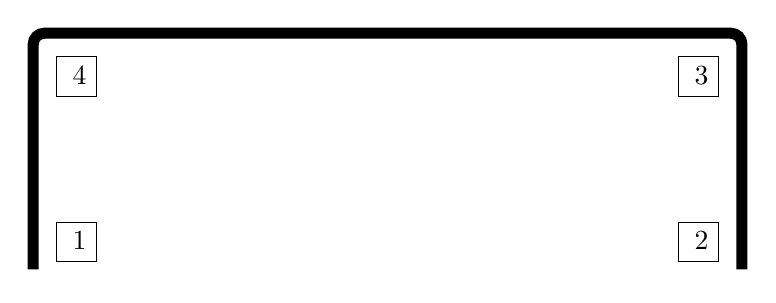
\begin{tikzpicture}[>=stealth]
\draw[line width =4pt, rounded corners] (0,0)--(0,3)--(9,3)--(9,0);
\draw (0.3,0.1) rectangle (0.8,0.6) node[below left]{$1$};
\draw (0.3,2.2) rectangle (0.8,2.7) node[below left]{$4$};
\draw (8.2,0.1) rectangle (8.7,0.6) node[below left]{$2$};
\draw (8.2,2.2) rectangle (8.7,2.7) node[below left]{$3$};

\end{tikzpicture}
\hspace*{-5.5cm}
\begin{tikzpicture}[y=0.80pt, x=0.80pt, yscale=-1, xscale=1, inner sep=0pt, outer sep=0pt,scale=0.9]
\begin{scope}[shift={(0,99.0)},xscale=0.100,yscale=-0.100,fill=black]
\path[fill] (480,862) .. controls (441,823) and
(441,787) .. (479,749) .. controls (507,722) and
(507,720) .. (485,726) .. controls (471,729) and
(446,723) .. (420,710) .. controls (364,681) and
(307,661) .. (245,646) .. controls (202,636) and
(195,631) .. (195,610) .. controls (195,587) and
(198,585) .. (235,589) .. controls (257,591) and
(304,603) .. (340,617) .. controls (376,630) and
(413,644) .. (423,647) .. controls (438,652) and
(440,643) .. (440,554) -- (440,456) --
(402,411) .. controls (348,347) and (344,336) ..
(336,241) .. controls (329,150) and (336,130) ..
(375,130) .. controls (408,130) and (417,147) ..
(424,231) .. controls (431,301) and (435,310) ..
(476,363) .. controls (501,394) and (527,420) ..
(533,420) .. controls (540,420) and (566,394) ..
(591,362) .. controls (635,308) and (637,301) ..
(644,226) .. controls (650,144) and (658,130) ..
(697,130) .. controls (732,130) and (739,156) ..
(729,253) .. controls (721,337) and (718,344) ..
(675,399) -- (630,456) -- (630,554) .. controls
(630,662) and (629,661) .. (702,624) .. controls
(740,605) and (849,580) .. (866,587) .. controls
(874,590) and (880,602) .. (878,613) .. controls
(876,629) and (862,636) .. (817,647) .. controls
(785,654) and (725,675) .. (683,695) .. controls
(641,714) and (600,730) .. (592,730) .. controls
(579,730) and (579,732) .. (592,748) .. controls
(618,776) and (622,807) .. (606,839) .. controls
(588,874) and (585,875) .. (543,885) .. controls
(515,891) and (506,887) .. (480,862) -- cycle;
\end{scope}

\end{tikzpicture}
\end{center}
\loigiai{
Gọi $A_i$ là biến cố cầu thủ sút vào vị trí $i$, $B_i$là biến cố thủ môn bay người đến vị trí $i$ ($i=1,2,3,4$). Dễ thấy $\mathrm{P}(A_i)=\mathrm{P}(B_i)=\dfrac{1}{4}$. Gọi $C$ là biến cố cú sút không vào lưới. Ta có
\begin{align*}
\mathrm{P}(C)=\mathrm{P}(A_1)\mathrm{P}(B_1)+ \mathrm{P}(A_2)\mathrm{P}(B_2) + \dfrac{1}{2}\mathrm{P}(A_3)\mathrm{P}(B_3)+ \dfrac{1}{2}\mathrm{P}(A_4)\mathrm{P}(B_4)=\dfrac{3}{16}=0{,}1875.
\end{align*}
}
\end{ex}
\Closesolutionfile{ans}
\Closesolutionfile{ansbook}